\documentclass[../dazhuan.tex]{subfiles}
\graphicspath{{../image/}}

\begin{document}
%\addcontentsline{toc}{part}{寸草春晖}
\clearpage
\pagestyle{empty}
\pdfbookmark[-1]{寸草春晖}{spring}
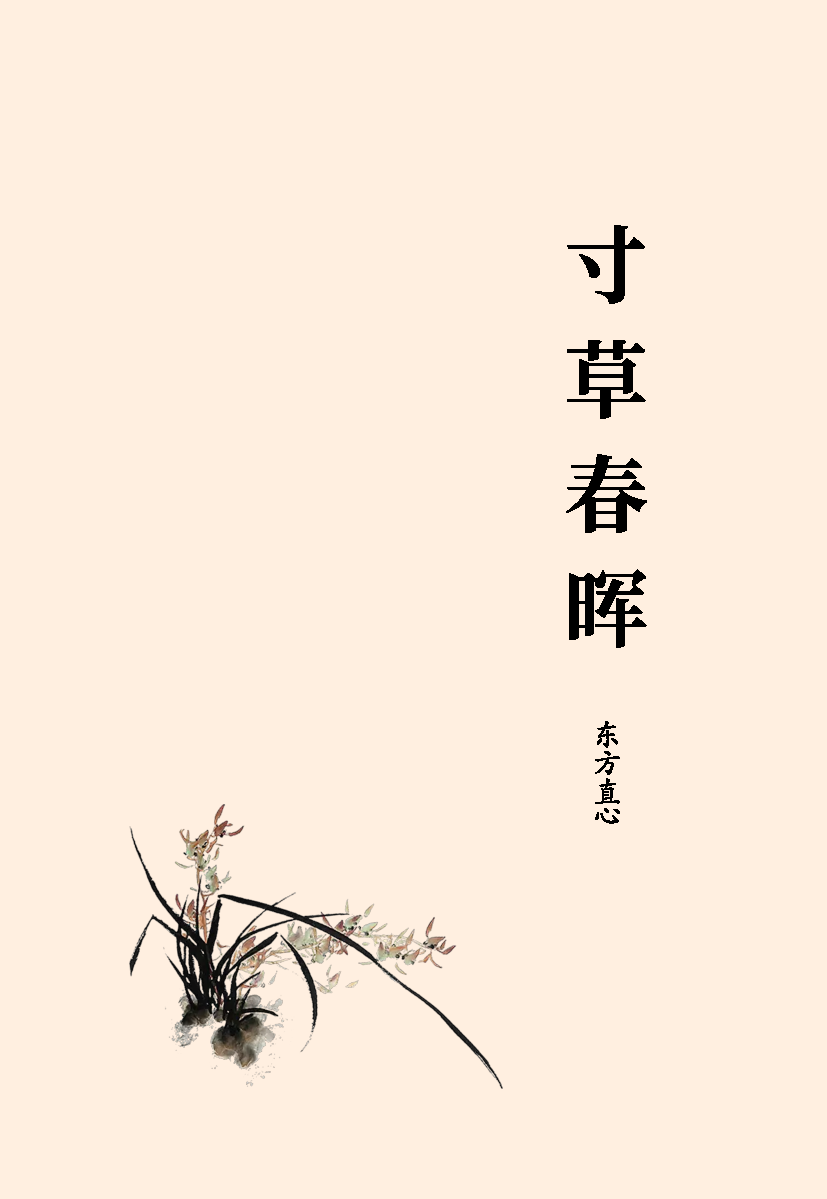
\includepdf{frontpage_add}
%\addcontentsline{toc}{part}{寸草春晖}
\tableofcontents[tod]

\pagestyle{plain}
\setcounter{page}{1}
\subfile{Z02/Z02C00} % 小序言
\subfile{Z02/Z02C01} % 我生之初
\subfile{Z02/Z02C02} % 沟北人
\subfile{Z02/Z02C03} % 曾祖母的功德
\subfile{Z02/Z02C04} % 不能忘怀的二伯父
\subfile{Z02/Z02C05} % 祖父绰号田二爷
\subfile{Z02/Z02C06} % 父亲和母亲【《挑夫泪》《祭母文》】
\subfile{Z02/Z02C07} % 奇闻轶事【(一)(二)(三)(四)(五)】
\subfile{Z02/Z02C08} % 苦乐童年【(一)(二)】
\subfile{Z02/Z02C09} % 兴趣爱好
\subfile{Z02/Z02C10} % 毛主席的客人
\subfile{Z02/Z02C11} % 从韶山到井冈山
\subfile{Z02/Z02C12} % 学校斗批改
\subfile{Z02/Z02C13} % 区总部
\subfile{Z02/Z02C14} % 两个总司令部
\subfile{Z02/Z02C15} % 大联合与三结合
\subfile{Z02/Z02C16} % 落幕前后
\subfile{Z02/Z02C17} % 从民工到武装民兵
\subfile{Z02/Z02C18} % 批林批孔宣讲团
\subfile{Z02/Z02C19} % 工农兵学员
\subfile{Z02/Z02C20} % 生存是未来的希望
\subfile{Z02/Z02C21} % 教书育人
\subfile{Z02/Z02C22} % 萍踪心语
\subfile{Z02/Z02C23} % 在历史脊背上划一个道道



\clearpage
\end{document}